\documentclass[lettersize,journal]{IEEEtran}
\usepackage{amsmath,amsfonts}
\usepackage{algorithmic}
\usepackage{algorithm}
\usepackage{array}
\usepackage[caption=false,font=normalsize,labelfont=sf,textfont=sf]{subfig}
\usepackage{textcomp}
\usepackage{stfloats}
\usepackage{url}
\usepackage{verbatim}
\usepackage{graphicx}
\usepackage{cite}
\usepackage{macros}
\usepackage{wrapfig}
\usepackage{subcaption}
\usepackage{hyperref}
\usepackage{adjustbox}
\usepackage{tikz}
\usepackage{multirow}






\usepackage[utf8]{inputenc}
\DeclareUnicodeCharacter{202F}{\,}  % map raw U+202F to a thin math‐space






\usetikzlibrary{automata, positioning, arrows}
\hyphenation{op-tical net-works semi-conduc-tor IEEE-Xplore}
% updated with editorial comments 8/9/2021

\newcounter{remarks}
\newtheorem{remark}{Remark}

\newcounter{examples}
\newtheorem{example}{Example}

\newcounter{definitions}
\newtheorem{definition}{Definition}

\newtheorem{note}{Note}




\begin{document}

%\subsection{Overview of the Proposed Approach}

\begin{figure}
	\centering
	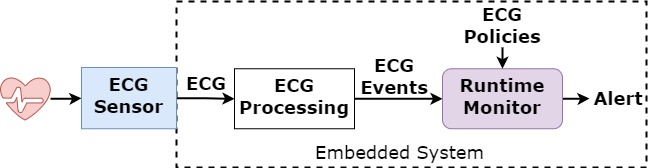
\includegraphics[width=0.5\textwidth]{Images/overview} 
	\caption{Proposed monitoring system}
	\label{monitoring_system}
\end{figure}


As seen in~\autoref{monitoring_system}, the electrical impulses of the human heart is captured by an ECG. The ECG signal is transformed into temporal events. We define policies on ECG features and specify them as timed automata (TA)~\cite{alur1994theory} which allows us to automatically synthesize an RV monitor. The monitor verifies if the incoming events satisfies the set of policies, and raises an alert if a policy is violated. Violation of policy indicates ECG/cardiac abnormality.

For the first time, we present specification, of ECG-based policies that identifies cardiac abnormalities, as TA. This enables us to synthesize formal verification monitors like RV. ECG policies and thus their TA specifications are based on Hampton's~\cite{hampton2019ecg} clinical interpretation of the primary cardiac abnormalities markers present in ECG.

%shows how the heart’s electrical impulses are recorded by an ECG. We define timed policies on ECG features to synthesize a runtime verification (RV) monitor that runs on a wearable device, classifies signals in real time, and raises an alert when abnormalities occur.

Key contributions:
\begin{itemize}
	\item We propose a formal RV monitor for classification of ECG
	enabling detection of cardiac abnormalities.
	\item We formalize ECG temporal features as a set of policies - specifying them as TA. The formally specified policies (as TA) are suitable for automated synthesis of an RV monitor.
	\item The proposed technique facilitates designing a wearable device for real-time ECG/cardiac monitoring.
	
	%\item Formalizing ECG timed features: Based on this, the set of policies based on ECG temporal features are formalized as Timed Automata (TA). The set of policies defined formally are suitable for automated analysis/synthesis of runtime monitors.
	
%	\item The proposed technique allows for designing a wearable
%	device for real-time health monitoring.
\end{itemize}
%\section{ECG Timed Policies}
\label{sec:ecgPolicies}
A typical ECG cycle has three main wave (P, QRS-complex and T waves)~\cite{hampton2019ecg}. We will use following temporal features to define our policies - PR, QRS-complex, QT, RR and P-wave intervals.

The P-wave interval is captured by the duration between \emph{onset} of P-peak and the \emph{offset} of P-peak. It represents atrial depolarization. The QRS-complex is the combined duration of Q, R and S waves. It represents ventricular depolarization. The PR interval is the duration between \emph{onset} of P-wave and the \emph{onset} of QRS-complex. It represents the time taken by the electrical impulse to travel from the atria to the ventricles. The time it taken for the ventricular depolarization-repolarization cycle is marked by the QT interval. It is the duration from the \emph{onset} of QRS-complex to the \emph{offset} T-wave. The RR interval, the interval between two successive R-waves of the ECG, is the diagnostic tool for heart rate and heart rate variability measurement.

We consider the following ECG timed safety policies (combined policy) for
developing the proposed classifier and thereby monitoring the abnormalities in
the heart~\cite{hampton2019ecg}.

\begin{itemize}
	\item $\varphi_{ECG1}$: The PR interval in ECG should be in the range of 120-200 ms.
	
	\item $\varphi_{ECG2}$: The QRS-complex interval in ECG should be in the range of 80-120 ms.
	
	\item $\varphi_{ECG3}$: The QTc interval in ECG should be between 350-480 ms.
	
	\item $\varphi_{ECG4}$: The RR interval in ECG should be in the range of 600-1200 ms.
	
	\item $\varphi_{ECG5}$: The P-wave interval in ECG should be less than or equal to 120 ms.
	
\end{itemize}


%The policy $\varphi_{ECG}$ = $\varphi_{ECG1}$ $\cap$ $\varphi_{ECG2}$ $\cdots$ $\cap$ $\varphi_{ECG5}$ represents the all the policies. The policies are formalized as timed automata, and thereby runtime monitors are synthesized that monitor these policies and raise the alarm in case of violations.


%\begin{note}
	\textit{Note:} A healthy individual may not adhere to the standard ECG temporal specifications (timing ranges) all the time, however repeated violations of these policies can be an early indication of severe cardiac issues and thus need continuous monitoring. Details about how heart abnormalities are captured by ECG timed policies is discussed here~\cite{appendiz}	
%\end{note}




%\section{Formal Specification of Policies and the RV Monitor}
This section briefly discusses timed automaton~\cite{alur1994theory}, specification of an ECG policy as TA, and explains the basics of a runtime verification monitor.
%%%%%%%%%%%%%%%%%%%%%%%%%%%%%%%%%%%%%%%%%%%%%%%%%%%
%\vspace{-1.5em}
\subsection{Timed Automata (TA)}
%\vspace{-0.5em} 
\begin{definition}[Timed automata]
	\label{def:ta}
	A {\em timed automaton} $\calA=(S, s_0, C, \Sigma,$ $\Delta, F)$ is a tuple, where:
	$S$ is a finite set of {\em locations}, $s_0 \in S$ is the \emph{initial location}, $C$ is a finite set of \emph{clocks}, $\Sigma$ is a finite set of {\em events}, $\Delta\subseteq S \times \mathcal{G}(C), \Sigma \times 2^C \times S$ is the {\em transition relation}, $F\subseteq S$ is a set of \emph{accepting locations}.	
\end{definition}
%%%%%%%%%%%%%%%%%%%%%%%%%%%%%%%%%%%%%%%%%%%%%%%%%%
%
%
\ignore{\vspace{-1.25em}
\begin{figure}[hbt!]
	\centering
	{
		\includegraphics[width=\linewidth]{fig/Policy_phi_1_c_true_c_false_page.jpg}
		\vspace{-1.5em}
		\caption{Policy $\varphi_{PAT1}$ represented by a timed automaton}
		\label{fig:exampleTA}
	}
	\vspace{-0.75em}
\end{figure}
\vspace{0.1em}}

\begin{figure}
	\begin{adjustbox}{width=\linewidth}
	
	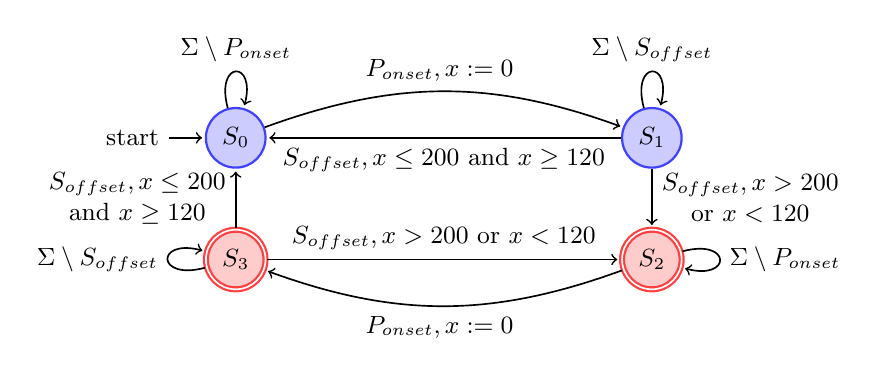
\begin{tikzpicture}[->,shorten >=1pt,auto,node distance=2.5cm,semithick,initial where=left]
		
		\tikzstyle{every node}=[font=\small]
		
		\tikzstyle{good state}=[circle,thick,draw=blue!75,fill=blue!20,minimum size=5mm]
		\tikzstyle{bad state}=[circle,thick,draw=red!75,fill=red!20,minimum size=3mm,accepting]
		\tikzstyle{dead state}=[rectangle,thick,draw=red!75,fill=red!20,minimum size=5mm]
		
		\node[initial,good state] (N0) {$S_0$};
		\node[good state]         (N1) [right=4.5 of N0] {$S_1$}; %[right of=N0] {$l_1$};
		\node[bad state]        (H) [below=0.75 of N1] {$S_2$};
		\node[bad state]        (H1) [below=0.75 of N0] {$S_3$};
		
		\path (N0) edge  [bend left=20] node [align=center]  {$ P_{onset}, x:=0 $ }( N1)
		
		%edge [loop above] node [align=center] {$ B_{G_1} $: $ b_1=1 $\\$C_{G_1}$: $ c_1=1 $}(N0)  
		edge [loop above] node [align=center] {$ \Sigma \setminus P_{onset} $}(N0)  
		%(H)edge [bend left=20] node [align=center] {$ R, x:=0 $ }(N1)          
		(N1)edge [bend left=0] node [align=center, pos=0.5, below] {$ S_{offset}, x\leq200 $ and $ x\geq120 $} (N0)
		(H1)edge node [align=center] {$ S_{offset}, x\leq200 $\\ and $ x\geq120 $} (N0)
		%(N1) edge  [loop right] node {$ A_{G_1} $} (N1)
		(N1)edge node [align=center] {$ S_{offset}, x>200 $  \\or $ x<120 $} (H)
		edge [loop above] node [align=center] {$ \Sigma \setminus S_{offset} $}(N1)
		%edge [loop above] node [align=center] {$ \Sigma \setminus on $}(H1)
		(H) edge [loop right] node {$ \Sigma \setminus P_{onset} $} (H)
		(H) edge  [bend left=20] node [align=center]  {$ P_{onset}, x:=0 $ }( H1)
		(H1)edge  [bend left=0] node [align=center, pos=0.5, above] {$ S_{offset}, x>200 $  or $ x<120 $} (H)
		edge [loop left] node [align=center] {$ \Sigma \setminus S_{offset} $}(H1);
		
	\end{tikzpicture}
		%content...
	\end{adjustbox}
	\caption{\red{Policy $\varphi_{ECG1}$ specified as TA.}}
	%\caption {figure} {VDTA specifying the constraint: ``\textit{Peer A can undertake a research project only after it has been approved by peer \{B, C\}}".}
	\label{fig:vdta}
\end{figure}

%\begin{example}
	\begin{example}[Timed automaton]
		%Let us consider the property $P_3$ discussed in Section \ref{sec:pacemaker}. The TA in Figure \ref{fig:policy1} represents policy $P_{ECG1}$ (i.e; The PR interval in ECG should be in the range  120-200 ms.). In the TA in Figure \ref{fig:policy1}, the set of locations is $L=\{s_0, s_1, s_2 \}$, where $s_0$ is the initial location, and $\Sigma$ = $\{ \mathit{P_{onset}}$, $\mathit{P_{offset}}$, $\mathit{QRS_{onset}}$, $\mathit{R}$, $\mathit{QRS_{offset}}$, $\mathit{T_{end}}  \}$ is the set of events. The set of real-valued clocks is $X = \{x\}$. Transitions occur between locations depending on events.  On the transitions, there are guards with constraints on clock values such as $x > 200$,  and resets of clocks ($x:=0$). When the first event $\mathit{P_{Onset}}$ occurs, the TA moves to $s_1$ from $s_0$, and the clock $x$ is reset to 0. When in location  $s_1$, if the event $\mathit{Q}$ occurs and if $  120 \leq  x \leq 200 $, then the TA remains in location $s_1$, and resets the value of clock $x$ to 0, otherwise, it moves to location $s_2$. The location $s_2$  (non-accepting) should never be reached for the policy to be satisfied over runs. 
		%
	\red{	Consider the policy $\varphi_{ECG1}$ mentioned in Section \ref{sec:ecg}: "The PR interval in ECG should be in the range 120-200 ms". The TA representing the policy is shown in Figure \ref{fig:policy1} where the set of locations in the TA is $S=\{s_0, s_1, s_2, s_3 \}$, with $s_0$ is the initial location, and the set of events is $\Sigma$ = $\{ \mathit{P_{onset}}$, $\mathit{P_{offset}}$, $\mathit{QRS_{onset}}$, $\mathit{R}$, $\mathit{QRS_{offset}}$, $\mathit{T_{end}} \}$. Here, there is a single clock $x$ ($C = \{x\}$ is the set of real-valued clocks) to measure the elapsed time between events. Depending on the events, transitions take place between places satisfying guards. In the TA, the guard $x$ $\geq$ 200, and clock resets ($x:=0$), are present on transitions. The clock $x$ is set to zero and the TA is moved to $s_1$ when the first event $\mathit{P_{offset}}$ takes place. If the event $\mathit{QRS_{offset}}$ occurs while the TA is in location $s_1$ and if the guard on the clock $x$ ($ 120 \leq x \leq 200 $) is satisfied, it stays in location $s_1$ and resets the value of clock $x$ to 0, otherwise it moves to the location $s_2$. The location $s_2$ (non-accepting) should never be reached to satisfy the policy over the runs. When in $s_2$, a $\mathit{P_{offset}}$ event triggers a transition to $s_3$ and resets $x$; if $\mathit{P_{offset}}$ does not occur, the TA remains in $s_2$. Then, upon a $\mathit{P_{offset}}$ event in $s_3$, if 120 $\leq$ x $\leq$ 200 holds, the TA returns to $s_0$; otherwise it transitions to $s_2$.}
	\end{example}
	The trace/timed word ($\sigma$) processed by the TA is a sequence of events along with time, for example, $\sigma=(e_1,t_1)\cdot(e_2, t_2)\cdots(e_n, t_n)$, where $e_i$ is an event and $t_i$ is the time of occurrence of the event. {Given a finite alphabet $\Sigma$, the set of timed words over $\Sigma$ is denoted by $\tw(\Sigma)$.}
	
%\end{example}
%%%%%%%%%%%%%%%%%%%%%%%%%%%%%%%%%%%%%%%%%
%\vspace{-1.5em}
\subsection{Runtime verification (RV) monitor}
%\vspace{-0.25em}
%%%%%%%%%%%%%%%%%%%%%%%%%%%%%%%%%%%%%%%%%%
\begin{definition}
	\label{def:rv:mon}
	Let $\varphi$ be a policy specified as TA $\calA_\varphi$. The RV monitor is a function $M_{\varphi}: \tw(\Sigma) \rightarrow \D$, where $\D= \{c\_True, c\_False\}$. Formally,
	\ignore{Consider a monitoring policy $\varphi\subseteq\tw(\Sigma)$ is formalized as a timed automata  $\calA_\varphi$, then the verification monitor synthesized from $\calA_\varphi$ can be represented as a function $M_{\varphi}: \tw(\Sigma) \rightarrow \D$, where $\D= \{c\_True, c\_False\}$. The RV monitor is defined as follows considering $\sigma \in \tw(\Sigma)$ as the current observation: }
	%%%%%%%%%%%%%%%%%%%%%%%%%%%%%%%%%%%%%%%%%
	\vspace{-0.5em}
	\[
	\begin{array}{lll}
		M_{\varphi}(\sigma) & =
		\begin{cases}
			c\_True & \mbox{if}\ \ \sigma\in\varphi \\%\wedge \exists \sigma'\in \tw(\Sigma): \sigma\cdot\sigma'\not\in\varphi \\
			c\_False & \mbox{if}\ \ \sigma\not\in\varphi %\wedge \exists \sigma'\in \tw(\Sigma): \sigma\cdot\sigma'\in\varphi \\
		\end{cases}
	\end{array}
	\]
\end{definition}
%%%%%%%%%%%%%%%%%%%%%%%%%%%%%%%%%%%%%%%%%
%\vspace{-0.5em}
The monitor $M_{\varphi}$ for the policy $\varphi$ takes $\sigma$ as input and emits a verdict from the set $D = \{c\_True, c\_False\}$, where $c\_True$ stands for \emph{currently true} and $c\_False$ for \emph{currently false}. It reads $\sigma$ event by event, and after each event, it emits $c\_True$ if $\sigma$ satisfies $\varphi$, $c\_False$ otherwise.
%After reading the timed word $\sigma$, if the policy is satisfied with the current observation, the monitor emits the verdict $c\_True$, otherwise, $c\_False$.
%\vspace{0.5em}



	
\begin{example}	
	Let's consider the policy $\varphi_{ECG}$ = $\varphi_{ECG1}$ $\cap$ $\cdots$ $\cap$ $\varphi_{ECG5}$ to monitor with a sample ECG trace. Let $(P_{onset},270)\cdot(P_{offset},350)\cdot(QRS_{onset},360)\cdot(R,420) \cdot (QRS_{offset}, 470) \cdot (T_{end}, 890)$ be the sample ECG input event sequence with the occurrence time (in ms). The RV monitor receives the trace, and each event is associated with a delay that represents the amount of time since the preceding event or the system initialization. Table \ref{tab:BPMon} displays the monitor's step-by-step behaviour.
	
	The first event $P_{onset}$ is received by the ECG monitor at $t=270$, and the monitor emits $C\_True$ because the policy is not violated. The event $P_{offset}$ is observed at $t=350$, and the monitor emits $C\_True$. (as P-wave duration is within a safe range and the policy is satisfied). The monitor will once again output $C\_True$ for the event $(QRS_{onset},360)$ because the PR interval is less than 200 ms, and the policy is not violated. The monitor emits $C\_True$ for the following event $(R,420)$ because the policy is satisfied. The monitor once more emits $C\_True$ because the QRS-complex duration is within a safe range, and there is no policy violation when the event $QRS_{offset}$ occurs at $t=470$. The policy is false for the event $(T_{end}, 890)$ since the QTc interval should be between 350 and 480 ms. As a result, the monitor will output the verdict $C\_False$, indicating that the currently observed trace violates the policy.	
\end{example}	
\ignore{
\begin{table*}[htb]
	\centering
	\caption{Example- Behavior of the RV monitor for policy $\varphi_{ECG1} \wedge  \cdots \wedge \varphi_{ECG5}$}	
	\vspace{-0.5em}
	\scalebox{0.9}{
		\begin{tabular}{|c|c|c|}
			\hline			$\sigma$ & $M_\varphi(\sigma)$   \\
			\hline
			$(P_{onset},270)$  & \ CT  \\
			\hline
			$(P_{onset},270)\cdot(P_{offset},350)$  & \ CT  \\
			\hline
			$(P_{onset},270)\cdot(P_{offset},350)\cdot(QRS_{onset},360) $   & \ CT \\
			\hline
			$(P_{onset},270)\cdot(P_{offset},350)\cdot(QRS_{onset},360)\cdot(R,420)$  & \ CT \\
			\hline
			$(P_{onset},270)\cdot(P_{offset},350)\cdot(QRS_{onset},360)\cdot(R,420) \cdot (QRS_{offset}, 470)$  & \ CT \\
			\hline			
			$(P_{onset},270)\cdot(P_{offset},350)\cdot(QRS_{onset},360)\cdot(R,420) \cdot (QRS_{offset}, 470), \cdot (T_{end},890)$ & \ CF \\
			\hline			
		\end{tabular}%
	}
	\label{tab:BPMon}%
	\vspace{-1.75em}	
\end{table*}}


%\section{Monitoring Cardiac Abnormalities/ECG}
In order to monitor all the policies discussed in~\autoref{sec:ecgPolicies}, we consider their intersection:  $\varphi_{ECG}$ = $\varphi_{ECG1}$ $\cap$ $\varphi_{ECG2}$ $\cdots$ $\cap$ $\varphi_{ECG5}$. Since each policy is formalized as TA, the intersection of these policies is defined as the product of TAs corresponding to each policy.

Given a policy $\varphi_{ECG}$ which corresponds to the product of the TAs, we synthesize an RV monitor $M_{\varphi_{ECG}}$ using the approach mentioned in~\cite{pinisetty2017predictive,pinisetty2018security,Bauer:2011:RVL}. The RV monitor inputs the sequence of temporal events (as timed word), and after each event provides a verdict whether $\varphi_{ECG}$ is satisfied (verdict = $c\_True$) or not (verdict = $c\_False$). It raises an alert when the verdict is \emph{currently false}, indicating abnormal behaviour in ECG.

\begin{example}
	%	
	%Let us consider policy $\varphi_{ECG}$ to be verified as the policy that we obtain by the intersection of policies $P_{ECG1}$, $\cdots$  \& $P_{ECG5}$ discussed earlier. The ECG monitor is invoked with its respective policy to verify an input event sequence (input sequence to be checked against the policy).
	%	
	%Let $(P_{onset},270)\cdot(P_{offset},350)\cdot(QRS_{onset},360)\cdot(R,420) \cdot (QRS_{offset}, 470) \cdot (T_{end}, 890)$ be an example of an ECG input event sequence along with the time (in ms) of occurrence. The trace is fed to the RV monitor, where each event is associated with a delay, indicating the time elapsed after the previous event or the system initialization. The step-wise behaviour of the monitor is shown in Table \ref{tab:BPMon}.
	%	
	%The ECG monitor receives the first event $P_{onset}$ at $t=270$ , the monitor emits $\ct$ as the policy is not violated. At $t=350$, the event $P_{offset}$ is observed, the monitor emits $\ct$ (as P-wave duration is within safe range and the policy is satisfied). For event $QRS_{onset}= 360$, the monitor will again emit verdict $\ct$ as the PR interval is within 200 ms, and the policy is not violated. For the next event $(R,420)$ , the monitor emits $\ct$ as there are no violated policies. When the event $QRS_{offset}$ comes at $t=470$, again the monitor emits $\ct$ as QRS duration is within a safe range and no violation of policies. For the event $(T_{end}, 890)$,  the policy is violated since the QTc interval should be within 350-480 ms. So, the monitor will output verdict $\cf$, indicating policy is violated by the currently observed trace.
	%
	Let's consider the policy $\varphi_{ECG}$ = $\varphi_{ECG1}$ $\cap$ $\cdots$ $\cap$ $\varphi_{ECG5}$ to monitor with a sample ECG trace. Let $(P_{onset},270)\cdot(P_{offset},350)\cdot(QRS_{onset},360)\cdot(R,420) \cdot (QRS_{offset}, 470) \cdot (T_{end}, 890)$ be the sample ECG input event sequence with the occurrence time (in ms). The RV monitor receives the trace, and each event is associated with a delay that represents the amount of time since the preceding event or the system initialization. Table \ref{tab:BPMon} displays the monitor's step-by-step behaviour.
	
	The first event $P_{onset}$ is received by the ECG monitor at $t=270$, and the monitor emits $C\_True$ because the policy is not violated. The event $P_{offset}$ is observed at $t=350$, and the monitor emits $C\_True$. (as P-wave duration is within a safe range and the policy is satisfied). The monitor will once again output $C\_True$ for the event $(QRS_{onset},360)$ because the PR interval is less than 200 ms, and the policy is not violated. The monitor emits $C\_True$ for the following event $(R,420)$ because the policy is satisfied. The monitor once more emits $C\_True$ because the QRS-complex duration is within a safe range, and there is no policy violation when the event $QRS_{offset}$ occurs at $t=470$. The policy is false for the event $(T_{end}, 890)$ since the QTc interval should be between 350 and 480 ms. As a result, the monitor will output the verdict $C\_False$, indicating that the currently observed trace violates the policy.
\end{example}	
%
%\vspace{-3.5em}
\begin{table}[htb]
	\centering
	\caption{\red{Example- Behavior of the RV monitor for policy $\varphi_{ECG1} \wedge  \cdots \wedge \varphi_{ECG5}$.}}	
	\vspace{-0.5em}
	%\scalebox{0.9}{
		\begin{adjustbox}{width=\columnwidth}
			
		\begin{tabular}{|c|c|c|}
			\hline			$\sigma$ & $M_\varphi(\sigma)$   \\
			\hline
			$(P_{onset},270)$  & \ct  \\
			\hline
			$(P_{onset},270)\cdot(P_{offset},350)$  & \ct  \\
			\hline
			$(P_{onset},270)\cdot(P_{offset},350)\cdot(QRS_{onset},360) $   & \ct \\
			\hline
			$(P_{onset},270)\cdot(P_{offset},350)\cdot(QRS_{onset},360)\cdot(R,420)$  & \ct \\
			\hline
			$(P_{onset},270)\cdot(P_{offset},350)\cdot(QRS_{onset},360)\cdot(R,420) \cdot (QRS_{offset}, 470)$  & \ct \\
			\hline			
			$(P_{onset},270)\cdot(P_{offset},350)\cdot(QRS_{onset},360)\cdot(R,420) \cdot (QRS_{offset}, 470), \cdot (T_{end},890)$ & \cf \\
			\hline			
		\end{tabular}%
		%content...
		\end{adjustbox}
	%}
	\label{tab:BPMon}%
	\vspace{-1.75em}	
\end{table}%
%\vspace{-0.5em}
%%%%%%%%%%%%%%%%%%%%%%%%%%%%%%%%%%%%%%%%%%
\ignore{
	\begin{remark}
		We assume the implicit resetting of the runtime monitor after every ECG cycle. As we are proposing continuous monitoring of ECG cycles to detect any cardiac abnormalities, when an ECG cycle violates a policy, the runtime monitor does not stop monitoring by waiting at the unsafe location of the TA. 
	\end{remark}
}
%\section{ECG Signal Processing}


\textit{ECG Dataset}: This work analyses the ECG records from the PTB-XL dataset \cite{wagner2020ptb}. The dataset consists of 21837 clinical 12-lead ECG records from 18885 patients, each of 10 seconds. It includes ECG from both men (52\%) and women (48\%) and spans the entire age range of 0 to 95 years. The collection includes a wide range of diagnostic classes, and cardiologists have annotated each ECG record. In this study, the policies are evaluated using lead II ECG readings (MLII).

%\textit{Preprocessing}: Generally, a raw ECG signal may be influenced by baseline wander, power line interference, noise, and artifacts. Hence, pre-processing of the signal is needed to filter unwanted data and extract vital information from the signals. We apply a band-pass Butterworth filter with 0.5 Hz and 40 Hz cutoff frequencies to remove baseline wander and noise from the input ECG signal.

\textit{Preprocessing}: Typically, a raw ECG signal can be distorted by several types of noise and artifacts. Hence, cleaning (preprocessing) the signal is therefore required to remove unnecessary data and obtain important information from the signals. To eliminate baseline wander and noise from the input ECG signal, a band-pass Butterworth filter with cutoff frequencies of 0.5 Hz and 40 Hz is employed.
%In this paper, the algorithm in [29] is used to bring the baseline drift to almost zero.

%\textit{Feature extraction}: After the filtering of the signal, the events of our interest are detected using the signal processing algorithm in python using the Neurokit2 tool \cite{makowski2021neurokit2}. The Pan-Tompkins algorithm \cite{pan1985real}) is used to detect the R-peak in the ECG signal. The other events such as $ \mathit{P_{onset}}, \mathit{P_{offset}}, \mathit{QRS_{onset}}, \mathit{QRS_{offset}}$ and $\mathit{T_{end}}  $ are extracted using discrete wavelet analysis implemented in Neurokit2 tool. 
%The \texttt{ECG\_Processing} module successfully detects all the relevant events for the recording. 
\textit{Feature extraction}: 
%Following the signal filtering, the events of our interest are found using the Neurokit2 tool's signal processing technique, which is implemented in Python. 
The R-peak in the ECG signal is located using the Pan-Tompkins technique \cite{pan1985real}) while we adapt the discrete wavelet analysis technique for extracting ECG events, such as $ \mathit{P_{onset}}, \mathit{P_{offset}}, \mathit{QRS_{onset}}, \mathit{QRS_{offset}}$ and $\mathit{T_{offset}} $ from an ECG signal.
%\section{\red{Implementation and Results}}


%\subsubsection{Implementation}
We implemented a two module prototype to showcase our method. The \texttt{ECG\_Processing} module (Python + NeuroKit2~\cite{makowski2021neurokit2}) reads signals from the PTB-XL dataset, applies peak detection and wavelet analysis, and emits sequence of time stamped events: $R_{peak}$, $P_{onset}$, $P_{offset}$, $QRS_{onset}$, $QRS_{offset}$, $QRS_{onset}$ , and $T_{onset}$, $T_{offset}$. These events are fed into the \texttt{RV\_Monitor} module (Python 2.7 + UPPAAL DBM~\cite{UPPAAL}), which loads the product automaton and, for each event, emits either $c\_True$ or $c\_False$.


%From PTB-XL we gathered a dataset of 30 individuals, each contributing a single ECG recording. Every ECG spans 10 seconds and is sampled at a rate of 100 Hz. As a result, we obtained 3000 data points, where each data point is classified as either currently true or currently false. We evaluate our model using three standard metrics:

From the PTB-XL database~\cite{wagner2020ptb}, we gathered a dataset consisting of ECG recordings from 30 individuals, each contributing a single ECG recording. Each ECG recording spans 10 seconds and is sampled at a rate of 100 Hz. As a result, we obtained 3000 data points per recording, where each data point is classified as either currently true or currently false. We evaluate our model using three standard metrics:

\ignore{\begin{align}
	\text{Accuracy} &= \frac{TP + TN}{TP + TN + FP + FN} \times 100\%, \\
	\text{Sensitivity} &= \frac{TP}{TP + FN} \times 100\%, \\
	\text{Specificity} &= \frac{TN}{TN + FP} \times 100\%,
\end{align}}

accuracy(\%) = (TP + TN)/(TP + TN + FP + FN) $\times$ 100

aensitivity(\%) = [TP/(TP + FN)] $\times$ 100

apecificity(\%) = [TN/(TN + FP)] $\times$ 100


where
	$TP$ denotes true positives,
	$TN$ denotes true negatives,
	$FP$ denotes false positives,
	$FN$ denotes false negatives.


The RV framework achieved an accuracy of $98.3\%$, a sensitivity of $98.6\%$, and a specificity of $98.5\%$.


%\subsubsection{Discussion}
Most ECG classification works, as shown in Table \ref{Table:previous works}, focus on arrhythmia detection and classification. The proposed RV framework efficiently classifies ECG traces with arrhythmia, atrial enlargement, bundle branch block, conduction issues, \etc (cf.~\cite{}). It may be noted that typical ECG traces can deviate from the standard specifications, but with repeated violations of the policies, the user gets an early warning.

%Most ECG classification works, as shown in Table \ref{Table:previous works}.This work considers policies to capture arrhythmia. The proposed RV framework efficiently classifies ECG traces with arrhythmia. It may be noted that typical ECG traces can deviate from the standard specifications, but with repeated violations of the policies, the user gets an early warning.

\begin{table}[]
	\centering
	\caption{\red{Few previous works.}}
	%\vspace{-0.5em}
	\begin{adjustbox}{width=\columnwidth}
	
	{
		\begin{tabular}{|c|c|c|c|c|c|c|}
			\hline
			Author             & \begin{tabular}[c]{@{}c@{}}Type of\\ classification\end{tabular} & Classes                                                    & ECG features                                                                                        & Database & Model & Accuracy \\ \hline
			Vijayavanan et al. \cite{vijayavanan2014automatic}& heart-beat                                                       & \begin{tabular}[c]{@{}c@{}}normal/\\ abnormal\end{tabular} & \begin{tabular}[c]{@{}c@{}}intervals- RR, PR, QT, ST, QRS duration,\\ segments- ST, PR\end{tabular} & MIT-BIH  & PNN   & 96.5     \\ \hline
			Tang and Shu \cite{tang2014classification}      & heart-beat                                                       & \begin{tabular}[c]{@{}c@{}}normal/\\ abnormal\end{tabular} & 3 angle features, 19 temporal features                                                              & MIT-BIH  & QNN   & 91.7     \\ \hline
			Zidelmal et al. \cite{zidelmal2013ecg}    & heart-beat                                                       & \begin{tabular}[c]{@{}c@{}}normal/\\ abnormal\end{tabular} & RR interval, QRS duration                                                                           & MIT-BIH  & SVM   & 98.8     \\ \hline
			Vishwa et al. \cite{vishwa2011clasification}      & heart-beat                                                       & \begin{tabular}[c]{@{}c@{}}normal/\\ abnormal\end{tabular} & RR interval                                                                                         & MIT-BIH  & ANN   & 96.7     \\ \hline
		\end{tabular}
	}
	%	content...
	\end{adjustbox}
	\label{Table:previous works}
	\vspace{-1.5em}
\end{table} 






%\input{content/conclusion}

%\section{Abstract}
%hypertension paper~\cite{DBLP:journals/esl/PandaAPR24}.
%\\


\section{CAPTURING HEART ABNORMALITIES AS TIMED AUTOMATA}

In the previous section, we discussed different conventional temporal
aspects of an ECG signal. In this section, we discuss the cardiac problems caused by temporal feature deviations and the timed policies
considered to monitor and classify ECG.
As previously stated, a typical ECG signal has various temporal
aspects, including PR, QT, RR, and P-wave intervals, as well as
conventional ranges. Any variations from these normal electrical
patterns can suggest a variety of heart conditions. Different ECG
waves and intervals, their usual ranges, and abnormalities in the heart

when these properties deviate from their safe ranges are presented in
Table \ref{table:abnormal}

\subsection{Capturing cardiac complications due to
	extended PR interval as TA}
	
Regular PR intervals average between 0.12 and 0.20 seconds. A
prolonged PR interval showing delayed transmission of the SA node
impulse to the ventricles is diagnostic of first-degree AV block. Firstdegree heart block is a clinically insignificant finding on its own;
however, heart diseases such as acute rheumatic carditis, an overdose
of digoxin, or an electrolyte imbalance may arise because of it. A
Harvard study found that people with PR intervals longer than 200
ms had an increased risk of atrial fibrillation, pacemaker insertion,
and premature death by roughly a factor of 1.5. Wolff-ParkinsonWhite and Lown-Ganong-Levine syndromes are two conditions in
which a short PR interval is seen because the heart is able to bypass
the AV node delay. The TA in Fig. \ref{fig:TA1} captures the extended PR
interval. The RV monitor raises the alarm whenever the standard PR
interval is violated, indicating the possibility of cardiac abnormalities
due to the prolonged PR interval.



\begin{table*}[]
	\centering
	\caption{ECG features and heart abnormalities}	
	\vspace{-0.5em}
	\resizebox{0.9\linewidth}{!}
	{	
		\begin{tabular}{|c|c|c|c|c|}
			\hline
			
			\begin{tabular}[c]{@{}c@{}}ECG waves\\  and\\ intervals\end{tabular} &
			\begin{tabular}[c]{@{}c@{}}Normal\\  Range\end{tabular} &
			\begin{tabular}[c]{@{}c@{}}Abnormal\\ duration\end{tabular} & Heart Abnormality 
			& References \\ \hline
			\multirow{2}{*}{PR interval}                                         &
			\multirow{2}{*}{0.12-0.20s}                             & $\le$ 0.12 s              
			& Pre-excitation syndromes                 
			& \cite{hampton2019ecg}         \\ \cline{3-5} 
			&                                                         & $\ge$ 0.2 s           
			& First-degree AV block                
			& \cite{hampton2019ecg}          \\ \hline
			\multirow{2}{*}{QRS complex}                                         &
			\multirow{2}{*}{0.08-0.12 s}                            & 0.1 - 0.12 s          
			& Incomplete bundle branch block         
			& \cite{hampton2019ecg}          \\ \cline{3-5} 
			&                                                         & $\ge$ 0.12 s          
			& Complete bundle branch block         
			& \cite{hampton2019ecg}         \\ \hline
			\multirow{2}{*}{QT interval}                                         &
			\multirow{2}{*}{350-480 ms}                             & $\ge$ 480 ms              
			& Abnormal ventricular repolarization                 
			& \cite{hampton2019ecg}        \\ \cline{3-5} 
			&                                                         & $\le$ 390 ms          
			& Abnormal ventricular depolarization or
			repolarization & \cite{hampton2019ecg}         \\ \hline
			RR interval                                                          & 0.6-1.2
			s                                               & variable                      
			& Irregular heart rhythm                           
			& \cite{hampton2019ecg}        \\ \hline
			
			P-wave                                                               & $\leq$
			0.12 s                                        & $\ge$ 0.12 s                               
			& atrial enlargement                                                 
			& \cite{hampton2019ecg}         \\ \hline
		\end{tabular}
	}
	\vspace{-1em}
	\label{table:abnormal}
\end{table*}


\begin{figure}
	\begin{adjustbox}{width=\linewidth}
		
		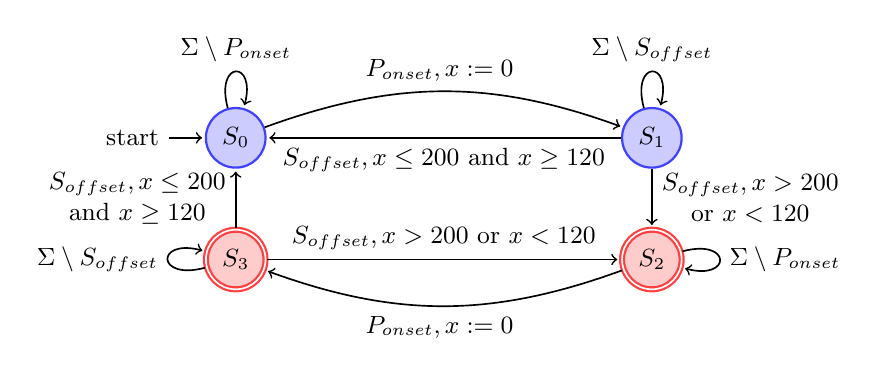
\begin{tikzpicture}[->,shorten >=1pt,auto,node distance=2.5cm,semithick,initial where=left]
			
			\tikzstyle{every node}=[font=\small]
			
			\tikzstyle{good state}=[circle,thick,draw=blue!75,fill=blue!20,minimum size=5mm]
			\tikzstyle{bad state}=[circle,thick,draw=red!75,fill=red!20,minimum size=3mm,accepting]
			\tikzstyle{dead state}=[rectangle,thick,draw=red!75,fill=red!20,minimum size=5mm]
			
			\node[initial,good state] (N0) {$S_0$};
			\node[good state]         (N1) [right=4.5 of N0] {$S_1$}; %[right of=N0] {$l_1$};
			\node[bad state]        (H) [below=0.75 of N1] {$S_2$};
			\node[bad state]        (H1) [below=0.75 of N0] {$S_3$};
			
			\path (N0) edge  [bend left=20] node [align=center]  {$ P_{onset}, x:=0 $ }( N1)
			
			%edge [loop above] node [align=center] {$ B_{G_1} $: $ b_1=1 $\\$C_{G_1}$: $ c_1=1 $}(N0)  
			edge [loop above] node [align=center] {$ \Sigma \setminus P_{onset} $}(N0)  
			%(H)edge [bend left=20] node [align=center] {$ R, x:=0 $ }(N1)          
			(N1)edge [bend left=0] node [align=center, pos=0.5, below] {$ S_{offset}, x\leq200 $ and $ x\geq120 $} (N0)
			(H1)edge node [align=center] {$ S_{offset}, x\leq200 $\\ and $ x\geq120 $} (N0)
			%(N1) edge  [loop right] node {$ A_{G_1} $} (N1)
			(N1)edge node [align=center] {$ S_{offset}, x>200 $  \\or $ x<120 $} (H)
			edge [loop above] node [align=center] {$ \Sigma \setminus S_{offset} $}(N1)
			%edge [loop above] node [align=center] {$ \Sigma \setminus on $}(H1)
			(H) edge [loop right] node {$ \Sigma \setminus P_{onset} $} (H)
			(H) edge  [bend left=20] node [align=center]  {$ P_{onset}, x:=0 $ }( H1)
			(H1)edge  [bend left=0] node [align=center, pos=0.5, above] {$ S_{offset}, x>200 $  or $ x<120 $} (H)
			edge [loop left] node [align=center] {$ \Sigma \setminus S_{offset} $}(H1);
			
		\end{tikzpicture}
		%content...
	\end{adjustbox}
	\caption{\red{Policy $\varphi_{ECG1}$ specified as TA.}}
	%\caption {figure} {VDTA specifying the constraint: ``\textit{Peer A can undertake a research project only after it has been approved by peer \{B, C\}}".}
	\label{fig:TA1}
\end{figure}


\subsection{ Capturing wide QRS complex as TA}

In general, the QRS-complex ranges between 0.08 and 0.10 seconds. When the time span is between 0.10 and 0.12 seconds, we
classify it as intermediate or prolonged QRS-complex. This may
indicate a left anterior or posterior fascicular block, or an incomplete right or left bundle branch block. When the QRS-complex
lasts longer than 0.12 seconds, medical attention is warranted. An
extended QRS duration is a symptom of a variety of heart rhythm
disorders, such as right bundle branch block, left bundle branch
block, non-specific intraventricular conduction delay, and ventricular arrhythmias such as ventricular tachycardia. Right-sided heart
problems are often indicated by a phenomenon known as right bundle branch block (RBBB). However, the left bundle branch block
(LBBB) is always associated with heart disease, most frequently
in the left ventricle. The prolonged QRS duration is captured by
the TA in Fig. \ref{TA2}. Every time the expected duration is exceeded, the
RV monitor sounds the alarm, warning of the potential for cardiac
problems caused by the prolonged QRS interval.

\begin{figure}
	\begin{adjustbox}{width=\linewidth}
		
		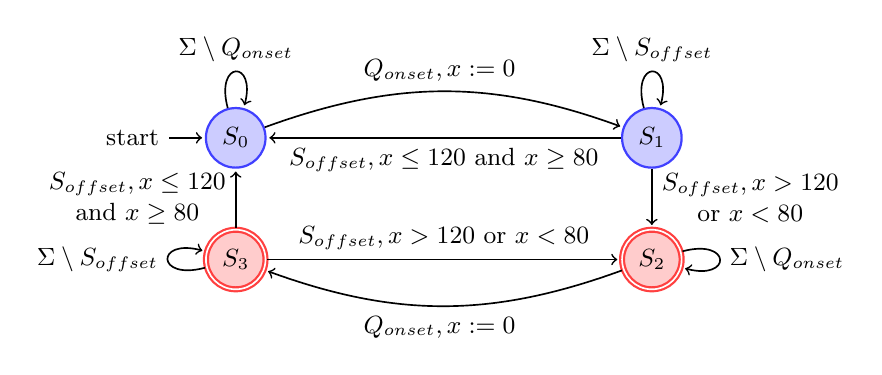
\begin{tikzpicture}[->,shorten >=1pt,auto,node distance=2.5cm,semithick,initial where=left]
			
			\tikzstyle{every node}=[font=\small]
			
			\tikzstyle{good state}=[circle,thick,draw=blue!75,fill=blue!20,minimum size=5mm]
			\tikzstyle{bad state}=[circle,thick,draw=red!75,fill=red!20,minimum size=3mm,accepting]
			\tikzstyle{dead state}=[rectangle,thick,draw=red!75,fill=red!20,minimum size=5mm]
			
			\node[initial,good state] (N0) {$S_0$};
			\node[good state]         (N1) [right=4.5 of N0] {$S_1$}; %[right of=N0] {$l_1$};
			\node[bad state]        (H) [below=0.75 of N1] {$S_2$};
			\node[bad state]        (H1) [below=0.75 of N0] {$S_3$};
			
			\path (N0) edge  [bend left=20] node [align=center]  {$ Q_{onset}, x:=0 $ }( N1)
			
			%edge [loop above] node [align=center] {$ B_{G_1} $: $ b_1=1 $\\$C_{G_1}$: $ c_1=1 $}(N0)  
			edge [loop above] node [align=center] {$ \Sigma \setminus Q_{onset} $}(N0)  
			%(H)edge [bend left=20] node [align=center] {$ R, x:=0 $ }(N1)          
			(N1)edge [bend left=0] node [align=center, pos=0.5, below] {$ S_{offset}, x\leq120 $ and $ x\geq80 $} (N0)
			(H1)edge node [align=center] {$ S_{offset}, x\leq120 $\\ and $ x\geq80 $} (N0)
			%(N1) edge  [loop right] node {$ A_{G_1} $} (N1)
			(N1)edge node [align=center] {$ S_{offset}, x>120 $  \\or $ x<80 $} (H)
			edge [loop above] node [align=center] {$ \Sigma \setminus S_{offset} $}(N1)
			%edge [loop above] node [align=center] {$ \Sigma \setminus on $}(H1)
			(H) edge [loop right] node {$ \Sigma \setminus Q_{onset} $} (H)
			(H) edge  [bend left=20] node [align=center]  {$ Q_{onset}, x:=0 $ }( H1)
			(H1)edge  [bend left=0] node [align=center, pos=0.5, above] {$ S_{offset}, x>120 $  or $ x<80 $} (H)
			edge [loop left] node [align=center] {$ \Sigma \setminus S_{offset} $}(H1);
			
		\end{tikzpicture}
		%content...
	\end{adjustbox}
	\caption{\red{Policy $\varphi_{ECG1}$ specified as TA.}}
	%\caption {figure} {VDTA specifying the constraint: ``\textit{Peer A can undertake a research project only after it has been approved by peer \{B, C\}}".}
	\label{fig:TA2}
\end{figure}

\subsection{Capturing prolonged QT interval as TA}

The QTc interval should be between 350 and 480 milliseconds. It is
prolonged in people with certain electrolyte disorders, and it is also
prolonged by some drugs. Ventricular tachycardia can be caused
by a prolonged QT interval (more than 480 ms). Long QT Interval
Syndromes occur when the QTc is larger than 480 ms (LQTS). This
condition has significant clinical implications because it typically suggests a higher risk of malignant ventricular arrhythmia, syncope,
and sudden death. Short QTc syndrome occurs when QTc is less than
0.35 s and can result in hypercalcemia and malignant arrhythmia.
The elongated QT interval is depicted by the TA in Fig. \ref{TA3}. When
the typical QT interval is exceeded, the RV monitor sounds an alert
because this may be a sign of cardiac problems.

\begin{figure}
	\begin{adjustbox}{width=\linewidth}
		
		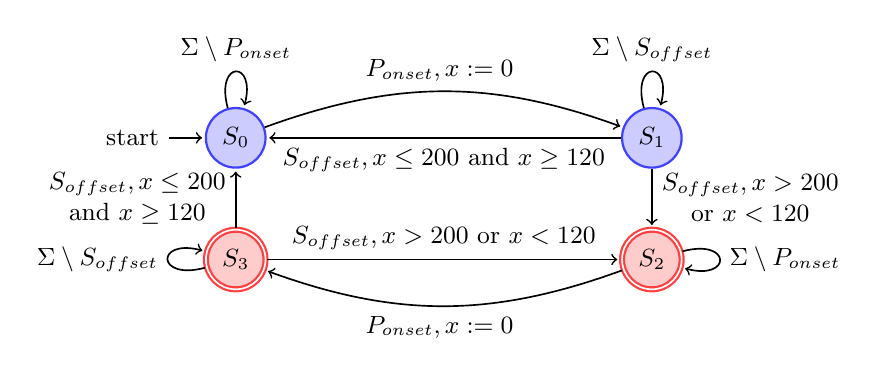
\begin{tikzpicture}[->,shorten >=1pt,auto,node distance=2.5cm,semithick,initial where=left]
			
			\tikzstyle{every node}=[font=\small]
			
			\tikzstyle{good state}=[circle,thick,draw=blue!75,fill=blue!20,minimum size=5mm]
			\tikzstyle{bad state}=[circle,thick,draw=red!75,fill=red!20,minimum size=3mm,accepting]
			\tikzstyle{dead state}=[rectangle,thick,draw=red!75,fill=red!20,minimum size=5mm]
			
			\node[initial,good state] (N0) {$S_0$};
			\node[good state]         (N1) [right=4.5 of N0] {$S_1$}; %[right of=N0] {$l_1$};
			\node[bad state]        (H) [below=0.75 of N1] {$S_2$};
			\node[bad state]        (H1) [below=0.75 of N0] {$S_3$};
			
			\path (N0) edge  [bend left=20] node [align=center]  {$ P_{onset}, x:=0 $ }( N1)
			
			%edge [loop above] node [align=center] {$ B_{G_1} $: $ b_1=1 $\\$C_{G_1}$: $ c_1=1 $}(N0)  
			edge [loop above] node [align=center] {$ \Sigma \setminus P_{onset} $}(N0)  
			%(H)edge [bend left=20] node [align=center] {$ R, x:=0 $ }(N1)          
			(N1)edge [bend left=0] node [align=center, pos=0.5, below] {$ S_{offset}, x\leq200 $ and $ x\geq120 $} (N0)
			(H1)edge node [align=center] {$ S_{offset}, x\leq200 $\\ and $ x\geq120 $} (N0)
			%(N1) edge  [loop right] node {$ A_{G_1} $} (N1)
			(N1)edge node [align=center] {$ S_{offset}, x>200 $  \\or $ x<120 $} (H)
			edge [loop above] node [align=center] {$ \Sigma \setminus S_{offset} $}(N1)
			%edge [loop above] node [align=center] {$ \Sigma \setminus on $}(H1)
			(H) edge [loop right] node {$ \Sigma \setminus P_{onset} $} (H)
			(H) edge  [bend left=20] node [align=center]  {$ P_{onset}, x:=0 $ }( H1)
			(H1)edge  [bend left=0] node [align=center, pos=0.5, above] {$ S_{offset}, x>200 $  or $ x<120 $} (H)
			edge [loop left] node [align=center] {$ \Sigma \setminus S_{offset} $}(H1);
			
		\end{tikzpicture}
		%content...
	\end{adjustbox}
	\caption{\red{Policy $\varphi_{ECG1}$ specified as TA.}}
	%\caption {figure} {VDTA specifying the constraint: ``\textit{Peer A can undertake a research project only after it has been approved by peer \{B, C\}}".}
	\label{fig:TA3}
\end{figure}


\subsection{Capturing wide P-wave as TA}

In addition, when the P-wave duration is longer than normal, it
usually indicates that one or both atria are enlarged (hypertrophied).
P waves can broaden or amplify as a result of atrial enlargements.
The shape of the P waves can be altered by ectopic atrial beats.
An absence of P waves is a characteristic of many abnormal heart
rhythms, such as atrial fibrillation and junctional arrhythmias. Short
RP can occur when the P waves are obscured by the end of the QRS
complex, as can happen in atrioventricular reentrant tachycardia.
The wide P-wave interval is depicted by the TA in the Fig. \ref{TA4}. When
the specified duration is exceeded, the RV monitor will sound the
alarm to alert the user to the fact that there is a potential for cardiac
irregularities as a result of the longer P-wave interval.

\begin{figure}
	\begin{adjustbox}{width=\linewidth}
		
		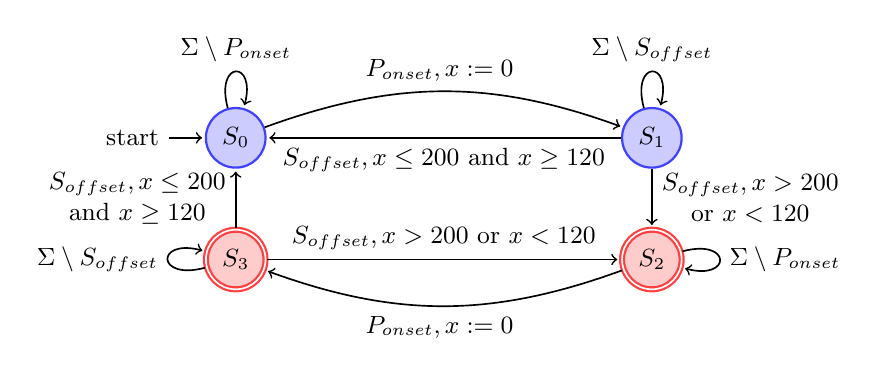
\begin{tikzpicture}[->,shorten >=1pt,auto,node distance=2.5cm,semithick,initial where=left]
			
			\tikzstyle{every node}=[font=\small]
			
			\tikzstyle{good state}=[circle,thick,draw=blue!75,fill=blue!20,minimum size=5mm]
			\tikzstyle{bad state}=[circle,thick,draw=red!75,fill=red!20,minimum size=3mm,accepting]
			\tikzstyle{dead state}=[rectangle,thick,draw=red!75,fill=red!20,minimum size=5mm]
			
			\node[initial,good state] (N0) {$S_0$};
			\node[good state]         (N1) [right=4.5 of N0] {$S_1$}; %[right of=N0] {$l_1$};
			\node[bad state]        (H) [below=0.75 of N1] {$S_2$};
			\node[bad state]        (H1) [below=0.75 of N0] {$S_3$};
			
			\path (N0) edge  [bend left=20] node [align=center]  {$ P_{onset}, x:=0 $ }( N1)
			
			%edge [loop above] node [align=center] {$ B_{G_1} $: $ b_1=1 $\\$C_{G_1}$: $ c_1=1 $}(N0)  
			edge [loop above] node [align=center] {$ \Sigma \setminus P_{onset} $}(N0)  
			%(H)edge [bend left=20] node [align=center] {$ R, x:=0 $ }(N1)          
			(N1)edge [bend left=0] node [align=center, pos=0.5, below] {$ S_{offset}, x\leq200 $ and $ x\geq120 $} (N0)
			(H1)edge node [align=center] {$ S_{offset}, x\leq200 $\\ and $ x\geq120 $} (N0)
			%(N1) edge  [loop right] node {$ A_{G_1} $} (N1)
			(N1)edge node [align=center] {$ S_{offset}, x>200 $  \\or $ x<120 $} (H)
			edge [loop above] node [align=center] {$ \Sigma \setminus S_{offset} $}(N1)
			%edge [loop above] node [align=center] {$ \Sigma \setminus on $}(H1)
			(H) edge [loop right] node {$ \Sigma \setminus P_{onset} $} (H)
			(H) edge  [bend left=20] node [align=center]  {$ P_{onset}, x:=0 $ }( H1)
			(H1)edge  [bend left=0] node [align=center, pos=0.5, above] {$ S_{offset}, x>200 $  or $ x<120 $} (H)
			edge [loop left] node [align=center] {$ \Sigma \setminus S_{offset} $}(H1);
			
		\end{tikzpicture}
		%content...
	\end{adjustbox}
	\caption{\red{Policy $\varphi_{ECG1}$ specified as TA.}}
	%\caption {figure} {VDTA specifying the constraint: ``\textit{Peer A can undertake a research project only after it has been approved by peer \{B, C\}}".}
	\label{fig:TA4}
\end{figure}

\subsection{Capturing variation in heartbeat as TA}

Variations in the RR interval have been extensively researched
in the context of irregular cardiac rhythm. The fluctuations in the
time intervals between individual heartbeats (R-peaks) are measured
by heart rate variability (HRV). The HRV can provide insights into
autonomic neural function as well as sympathetic-parasympathetic
autonomic balance and cardiovascular health ([13]). The extended
RR interval is captured by the TA in Fig. \ref{TA5}. Every time the normal
RR interval is violated, the RV monitor sounds the alarm, potentially
alerting the patient to the likelihood of cardiac problems caused by
the prolonged RR interval.


\begin{figure}
	\begin{adjustbox}{width=\linewidth}
		
		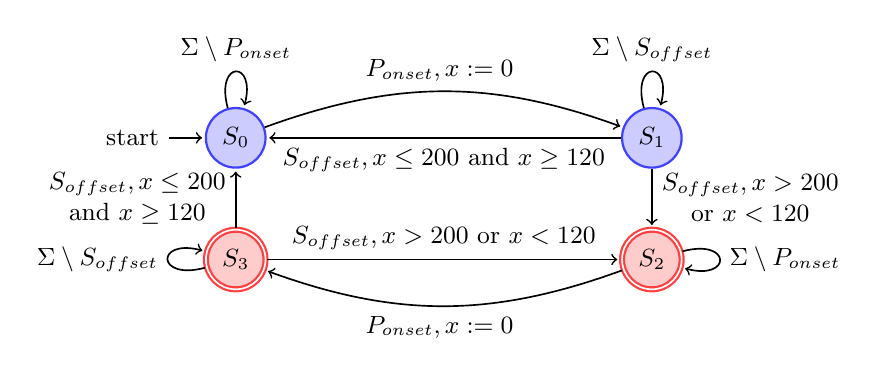
\begin{tikzpicture}[->,shorten >=1pt,auto,node distance=2.5cm,semithick,initial where=left]
			
			\tikzstyle{every node}=[font=\small]
			
			\tikzstyle{good state}=[circle,thick,draw=blue!75,fill=blue!20,minimum size=5mm]
			\tikzstyle{bad state}=[circle,thick,draw=red!75,fill=red!20,minimum size=3mm,accepting]
			\tikzstyle{dead state}=[rectangle,thick,draw=red!75,fill=red!20,minimum size=5mm]
			
			\node[initial,good state] (N0) {$S_0$};
			\node[good state]         (N1) [right=4.5 of N0] {$S_1$}; %[right of=N0] {$l_1$};
			\node[bad state]        (H) [below=0.75 of N1] {$S_2$};
			\node[bad state]        (H1) [below=0.75 of N0] {$S_3$};
			
			\path (N0) edge  [bend left=20] node [align=center]  {$ P_{onset}, x:=0 $ }( N1)
			
			%edge [loop above] node [align=center] {$ B_{G_1} $: $ b_1=1 $\\$C_{G_1}$: $ c_1=1 $}(N0)  
			edge [loop above] node [align=center] {$ \Sigma \setminus P_{onset} $}(N0)  
			%(H)edge [bend left=20] node [align=center] {$ R, x:=0 $ }(N1)          
			(N1)edge [bend left=0] node [align=center, pos=0.5, below] {$ S_{offset}, x\leq200 $ and $ x\geq120 $} (N0)
			(H1)edge node [align=center] {$ S_{offset}, x\leq200 $\\ and $ x\geq120 $} (N0)
			%(N1) edge  [loop right] node {$ A_{G_1} $} (N1)
			(N1)edge node [align=center] {$ S_{offset}, x>200 $  \\or $ x<120 $} (H)
			edge [loop above] node [align=center] {$ \Sigma \setminus S_{offset} $}(N1)
			%edge [loop above] node [align=center] {$ \Sigma \setminus on $}(H1)
			(H) edge [loop right] node {$ \Sigma \setminus P_{onset} $} (H)
			(H) edge  [bend left=20] node [align=center]  {$ P_{onset}, x:=0 $ }( H1)
			(H1)edge  [bend left=0] node [align=center, pos=0.5, above] {$ S_{offset}, x>200 $  or $ x<120 $} (H)
			edge [loop left] node [align=center] {$ \Sigma \setminus S_{offset} $}(H1);
			
		\end{tikzpicture}
		%content...
	\end{adjustbox}
	\caption{\red{Policy $\varphi_{ECG1}$ specified as TA.}}
	%\caption {figure} {VDTA specifying the constraint: ``\textit{Peer A can undertake a research project only after it has been approved by peer \{B, C\}}".}
	\label{fig:TA5}
\end{figure}










\section{Execution time}

\textit{Execution time:} Additionally, we investigated how long the runtime monitor took to process a cycle of an ECG. \footnote {Since the policies are independent, the RV monitors for each policy may be executed in parallel. In this experiment, we have explored the sequential execution of the RV monitors for each policy. In this case, dividing the total time indicated above by the number of monitors would give the overall execution time.} The average execution times for the RV monitor and the ECG processing module across several runs are shown in Table \ref{tab:performance} (approximately 1000 runs). For an ECG cycle, it takes the ECG processing module about 207.80 ms to find desired ECG events. The execution time for the combined policy is around 321 ms for an ECG cycle trace. We can see from the Table \ref{tab:performance} that the ECG processing module and RV monitor module take roughly 528.80 ms to complete one ECG cycle. Since an ECG cycle lasts roughly 1000-1200 ms, the RV framework is incredibly quick to report any ECG irregularities and identify any heart issues.
\vspace{-0.5em}
\begin{table}[!htb]
	\begin{minipage}{1\linewidth}
		\centering
		\caption{Accuracy of the RV monitor}
		\vspace{-0.5em}
		\resizebox{1\columnwidth}{!}
		{
			\begin{tabular}{|l|l|c|c|}
				\hline
				\multicolumn{1}{|c|}{Database} & \multicolumn{1}{c|}{ECG Record} & Status              & RV accuracy/cycle  \\ \hline
				PTB-XL                         & 03-3332                     & conduction issues   & 100\%   \\ \hline
				PTB-XL                         & 04-4546                     & bundle branch block & 70\%     \\ \hline
				PTB-XL                         & 04-4546                     & atrial enlargement  & 70\%     \\ \hline
				PTB-XL                        & 04-4469                     & sinus arrhythmia          & 100\%   \\ \hline
				PTB-XL                        & 04-4387                     & AV-block         & 100\%    \\ \hline
				PTB-XL                        & 04-06150                     & myocardial infarction         & 100\%    \\ \hline
			\end{tabular}
		}
		\label{table:accuracy}
	\end{minipage}
	%\vspace{-2em}
\end{table}
\vspace{-1.5em}
\begin{table}[!htb]
	\begin{minipage}{1\linewidth}
		\centering
		\caption{Execution time of the RV monitor}
		\vspace{-0.5em}
		\resizebox{\columnwidth}{!}
		{
			\begin{tabular}{|c|c|c|c|c|}
				\hline
				Policy &
				
				\begin{tabular}[c]{@{}c@{}}No. \\ of\\ ECG \\ cycles\end{tabular} &
				\begin{tabular}[c]{@{}c@{}}ECG\\  processing\\  Time (ms)\end{tabular} &
				\begin{tabular}[c]{@{}c@{}}ECG \\ RV monitor\\  Time (ms)\end{tabular}  &
				\begin{tabular}[c]{@{}c@{}} \\ Total \\  Time (ms)\end{tabular} 
				\\ \hline
				$P_{ECG1}$   & 1 & 207.80 & 15.175 & 222.255   \\ \hline
				$P_{ECG1}\& P_{ECG2}$   & 1 & 207.80 & 52.175 & 259.255   \\ \hline
				
				$P_{ECG1} \cdots  P_{ECG3}$   & 1 & 207.80 & 321 & 528.80   \\ \hline	
				$P_{ECG1} \cdots  P_{ECG4}$   & 1 & 207.80 & 321 & 528.80   \\ \hline
				$P_{ECG1} \cdots  P_{ECG5}$   & 1 & 207.80 & 321 & 528.80   \\ \hline
			\end{tabular}%
		}
		\label{tab:performance}
	\end{minipage}\hfill
	\vspace{-0.5em}
\end{table}
%>>>>>>> 1bc427e7d9925d29cd17e36eff3fd8e3b4b6eadf

\bibliographystyle{IEEEtran}
\bibliography{biblio}

\end{document}


